\let\negmedspace\undefined
\let\negthickspace\undefined
\documentclass[journal]{IEEEtran}
\usepackage[a5paper, margin=10mm, onecolumn]{geometry}
%\usepackage{lmodern} % Ensure lmodern is loaded for pdflatex
\usepackage{tfrupee} % Include tfrupee package

\setlength{\headheight}{1cm} % Set the height of the header box
\setlength{\headsep}{0mm}     % Set the distance between the header box and the top of the text

\usepackage{gvv-book}
\usepackage{gvv}
\usepackage{cite}
\usepackage{amsmath,amssymb,amsfonts,amsthm}
\usepackage{algorithmic}
\usepackage{graphicx}
\usepackage{textcomp}
\usepackage{xcolor}
\usepackage{txfonts}
\usepackage{listings}
\usepackage{enumitem}
\usepackage{mathtools}
\usepackage{gensymb}
\usepackage{comment}
\usepackage[breaklinks=true]{hyperref}
\usepackage{tkz-euclide} 
\usepackage{listings}
% \usepackage{gvv}                                        
\def\inputGnumericTable{}                                 
\usepackage[latin1]{inputenc}                                
\usepackage{color}                                            
\usepackage{array}                                            
\usepackage{longtable}                                       
\usepackage{calc}                                             
\usepackage{multirow}                                         
\usepackage{hhline}                                           
\usepackage{ifthen}                                           
\usepackage{lscape}
\begin{document}

\bibliographystyle{IEEEtran}
\vspace{3cm}

\title{10.5.3.9}
\author{EE23BTECH11063 - Yellanki Siddhanth
}
% \maketitle
% \newpage
% \bigskip
{\let\newpage\relax\maketitle}

\renewcommand{\thefigure}{\theenumi}
\renewcommand{\thetable}{\theenumi}
\setlength{\intextsep}{10pt} % Space between text and floats


\numberwithin{equation}{enumi}
\numberwithin{figure}{enumi}
\renewcommand{\thetable}{\theenumi}


\textbf{Question}:\\
Plot the points \brak{x,y} in Table 1.2.29
\begin{table}[h!]    
  \centering
  

  \caption{}
\end{table}\\


\textbf{Solution: }\\
  Let us first define the points:
  \begin{align}
    A \Rightarrow \myvec{-2 \\ 8}
  \end{align}
  \begin{align}
    B \Rightarrow \myvec{-1 \\ 7}
  \end{align}
  \begin{align}
    C \Rightarrow \myvec{0 \\ -1.25}
  \end{align}
  \begin{align}
    D \Rightarrow \myvec{1 \\ 3}
  \end{align}
  \begin{align}
    E \Rightarrow \myvec{3 \\ -1}
  \end{align}
    \begin{figure}[h]
        \centering
       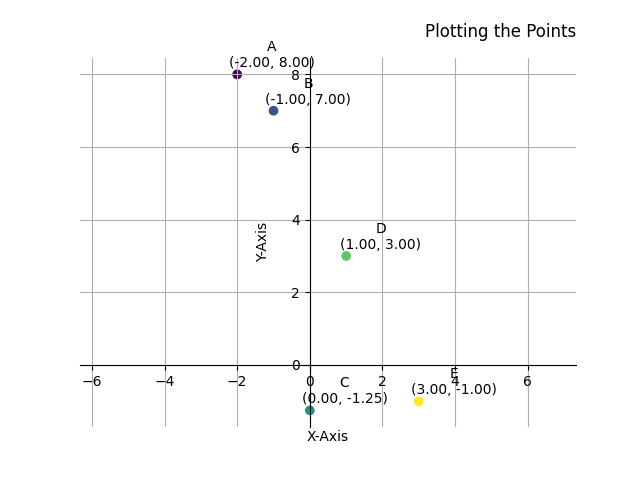
\includegraphics[width=0.7\linewidth]{figs/fig1.png}
       \caption{}
       \label{graph}
    \end{figure}
\end{document}  
\end{document}


